% !TEX program = xelatex
\documentclass[a4paper]{article}
\usepackage{amsmath}
\usepackage{amsthm}
\usepackage[left=1.8cm,right=1.8cm,top=2.2cm,bottom=2.0cm]{geometry}
\usepackage{ctex}
\usepackage{enumerate}
\usepackage{fancyhdr}
\usepackage{xpatch}
\usepackage{graphicx} 
\usepackage{float} 
\usepackage{subfigure} 
\usepackage{amsfonts}
\usepackage{mathtools}
\usepackage{framed}
\usepackage{multicol}
\usepackage{listings}
\usepackage{hyperref}
\usepackage{tikz}
\usetikzlibrary{automata,positioning}
\theoremstyle{definition}
\newtheorem*{solution*}{\textbf{Solution:}}
\newtheorem*{proof*}{\textbf{Proof:}}
\newtheorem{theorem}{Theorem}[subsection]
\newtheorem{definition}{Definition}[subsection]
\newtheorem{lemma}{Lemma}[subsection]
\makeatletter

\AtBeginDocument{\xpatchcmd{\@thm}{\thm@headpunct{.}}{\thm@headpunct{}}{}{}}
\makeatother

\pagestyle{fancy}
\renewcommand{\baselinestretch}{1.15}

\usepackage{paralist}
\let\itemize\compactitem
\let\enditemize\endcompactitem
\let\enumerate\compactenum
\let\endenumerate\endcompactenum
\let\description\compactdesc
\let\enddescription\endcompactdesc

% shorten footnote rule
\xpatchcmd\footnoterule
  {.4\columnwidth}
  {1in}
  {}{\fail}

\title{CS 131 Compilers: Discussion 6: Introduction to Modern Intermediate Representation}
\author{\textbf{杨易为}~~\textbf{季杨彪}~~\textbf{尤存翰} \\ \texttt{ \{yangyw,jiyb,youch\}@shanghaitech.edu.cn}}


\begin{document}
\maketitle
\section{Reusable IR}
\begin{enumerate}
   \item Modern compilers are made from loosely coupled components. 
   \item Front ends produce IR, AST as well. Thus they have to maintain all the information on Basic Block.
   \item Middle ‘ends’ transform IR (optimisation / analysis / instrumentation)
   \item Back ends generate native code (object code or assembly)
 \end{enumerate}

 \begin{center}
  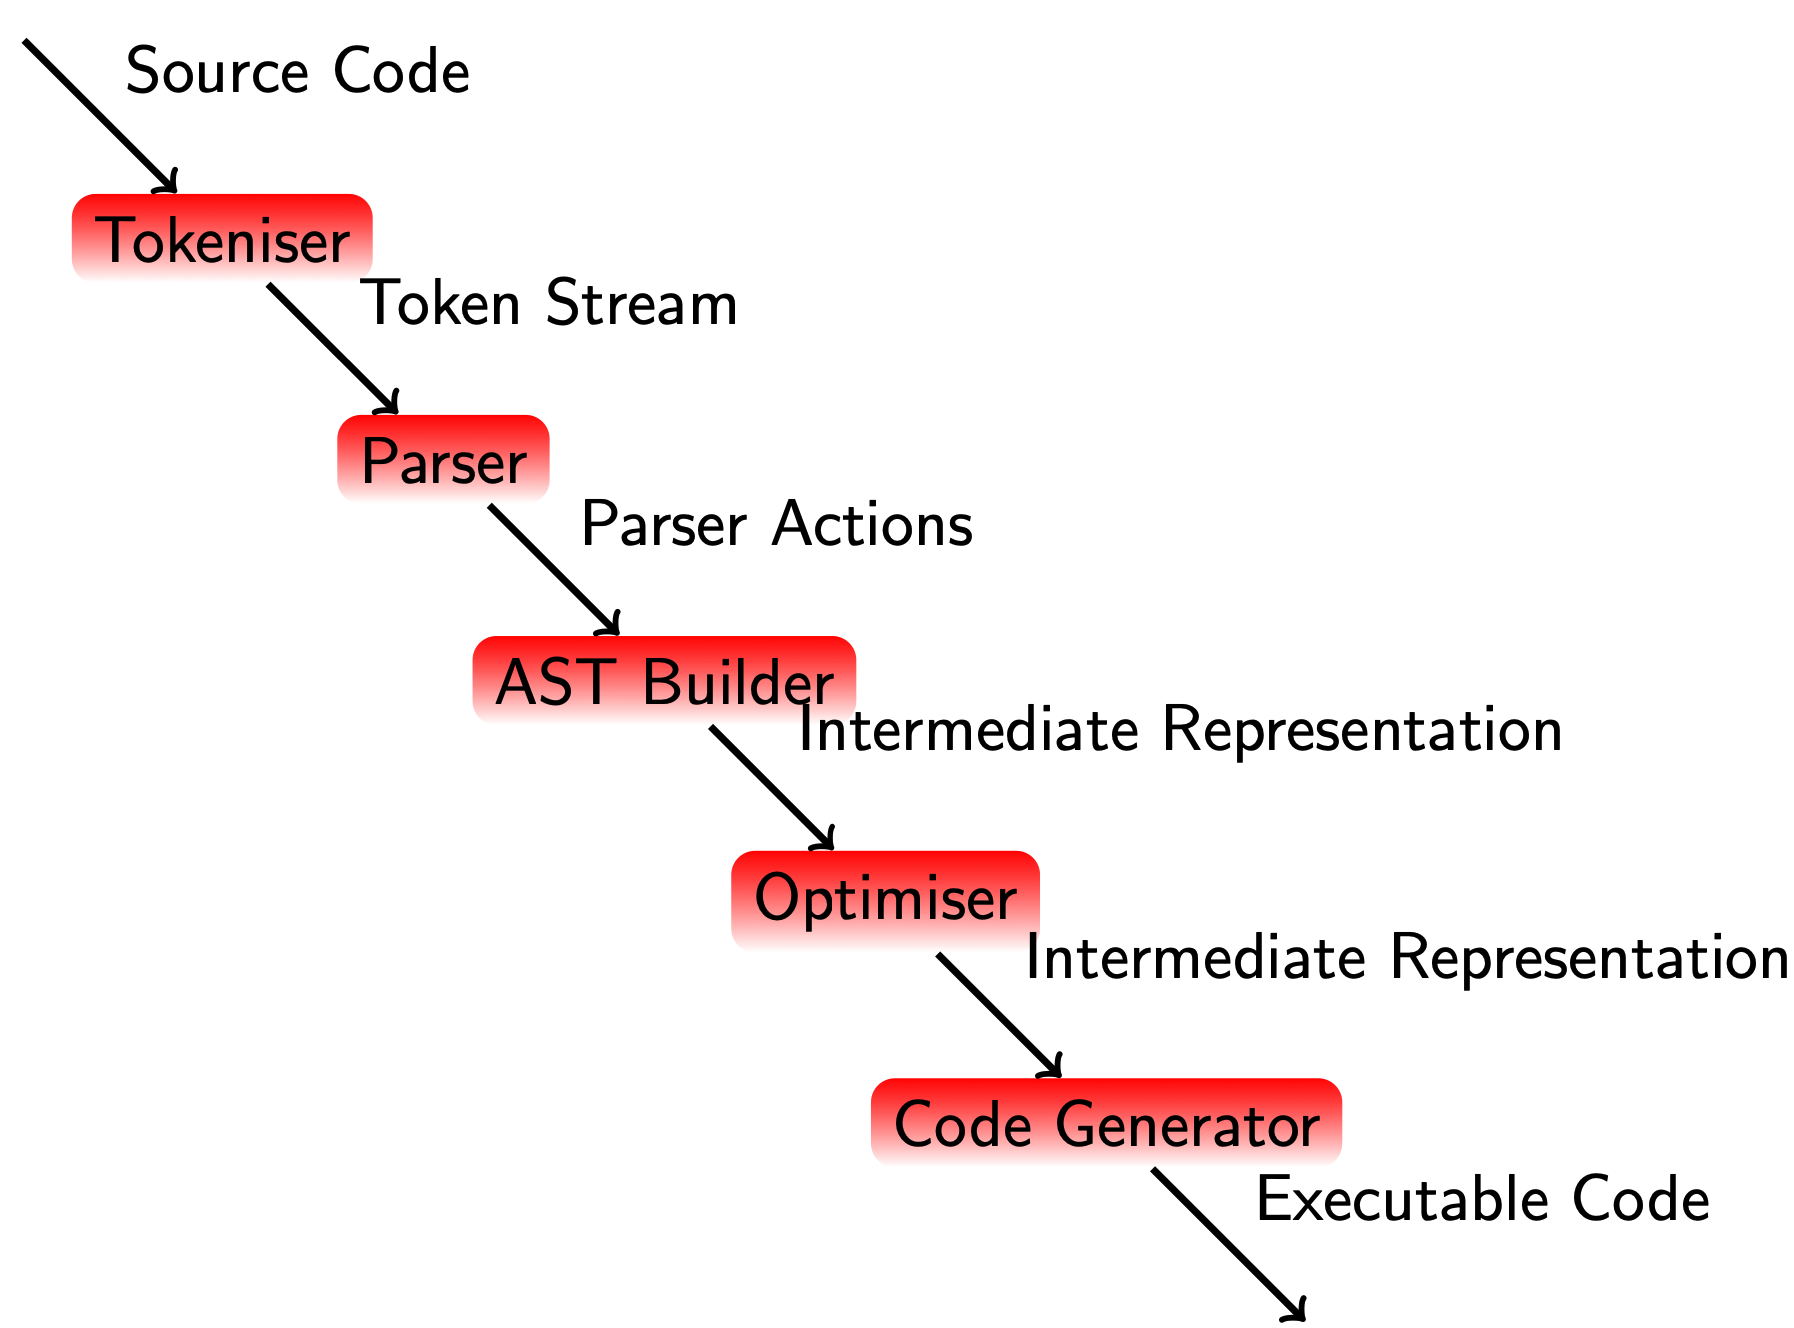
\includegraphics[height=3cm]{img/Snipaste_2021-04-05_17-18-11.png}
  \end{center}
  
  As with any other piece of software using libraries simplifies development.
  
  \subsection{Optimisation Passes}
  \begin{enumerate}
    \item  Modular, transform IR (Analysis passes just inspect IR)
    \item Can be run multiple times, in di↵erent orders
    \item May not always produce improvements when run in the wrong order!
    \item Some intentionally pessimise code to make later passes work better
  \end{enumerate}
  
  \subsection{Register vs Stack IR}
  \begin{enumerate}
    \item Stack makes interpreting, naive compilation easier • Register makes various optimisations easier
    \item Which ones?
  \end{enumerate}
  \begin{center}
   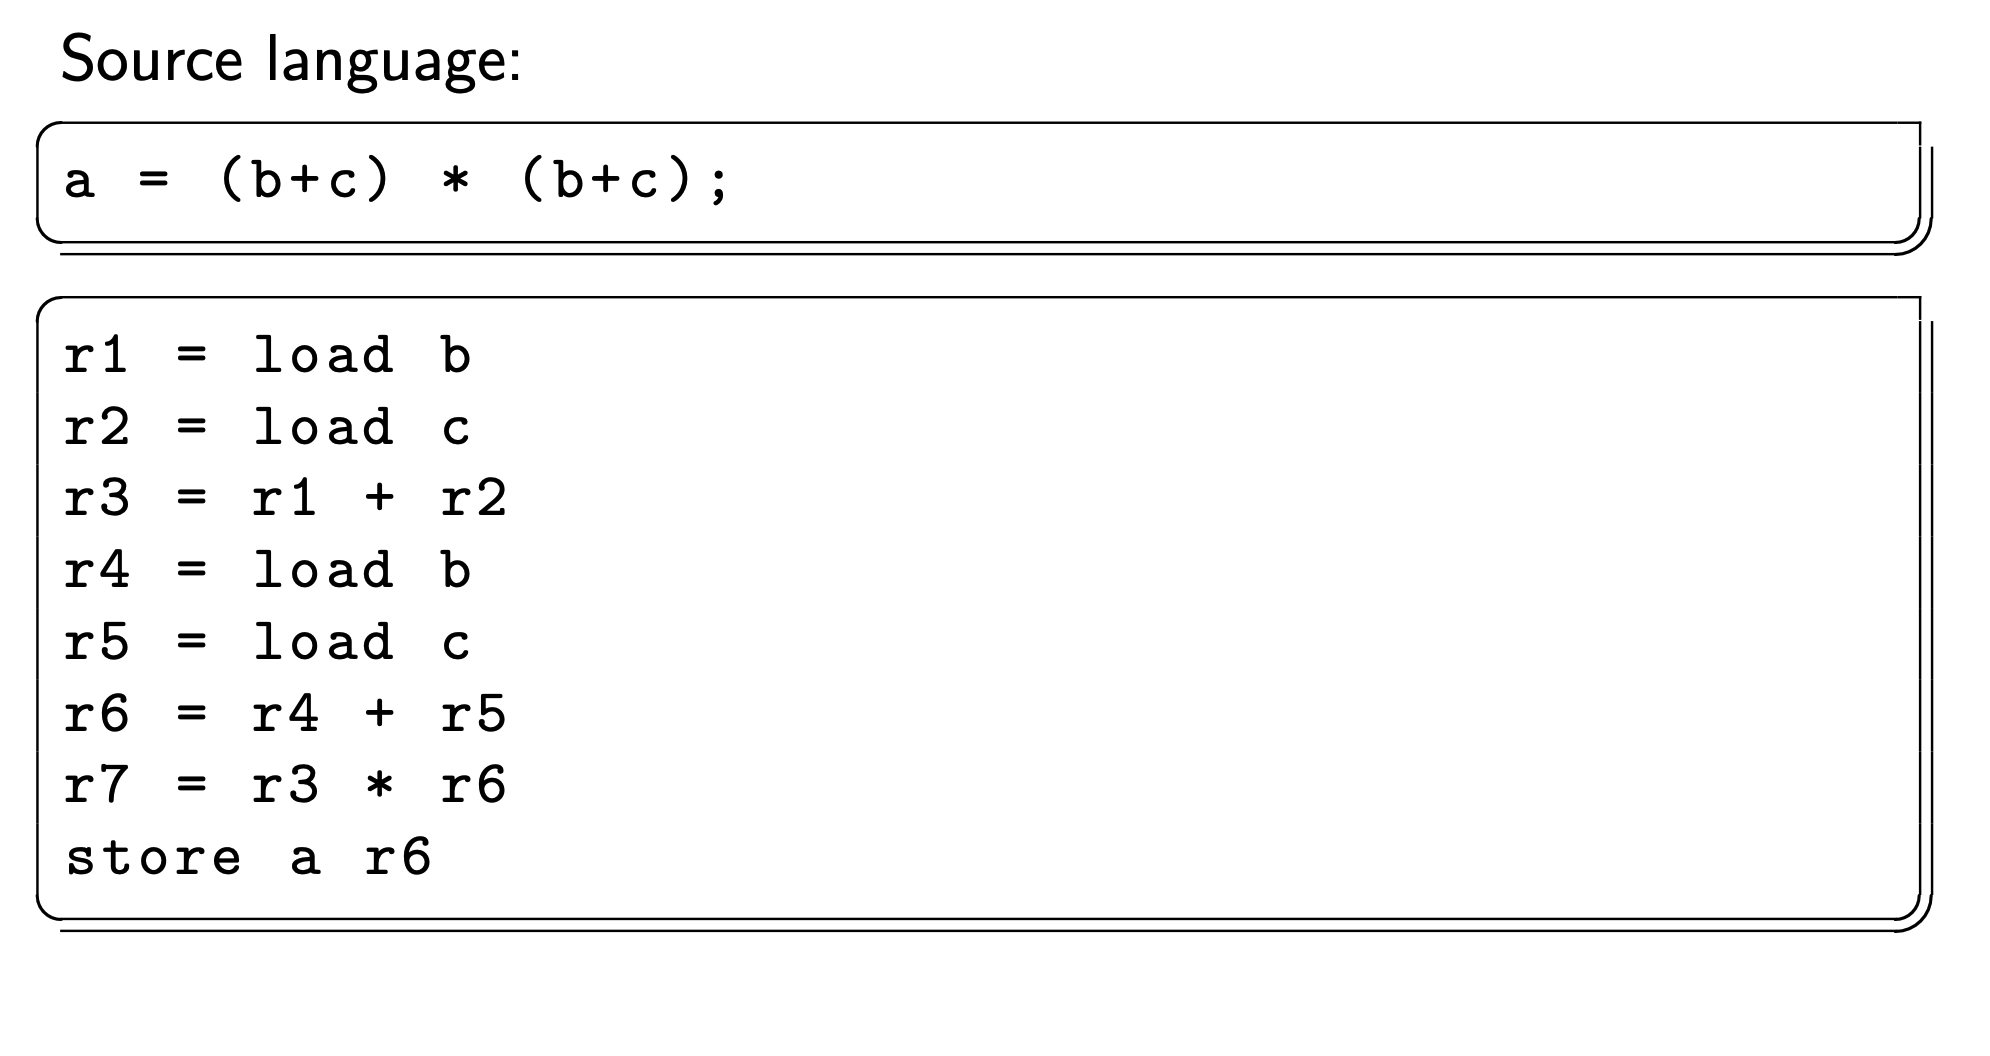
\includegraphics[height=3cm]{img/Snipaste_2021-04-05_17-25-13.png}
   \end{center}
   
  \begin{center}
   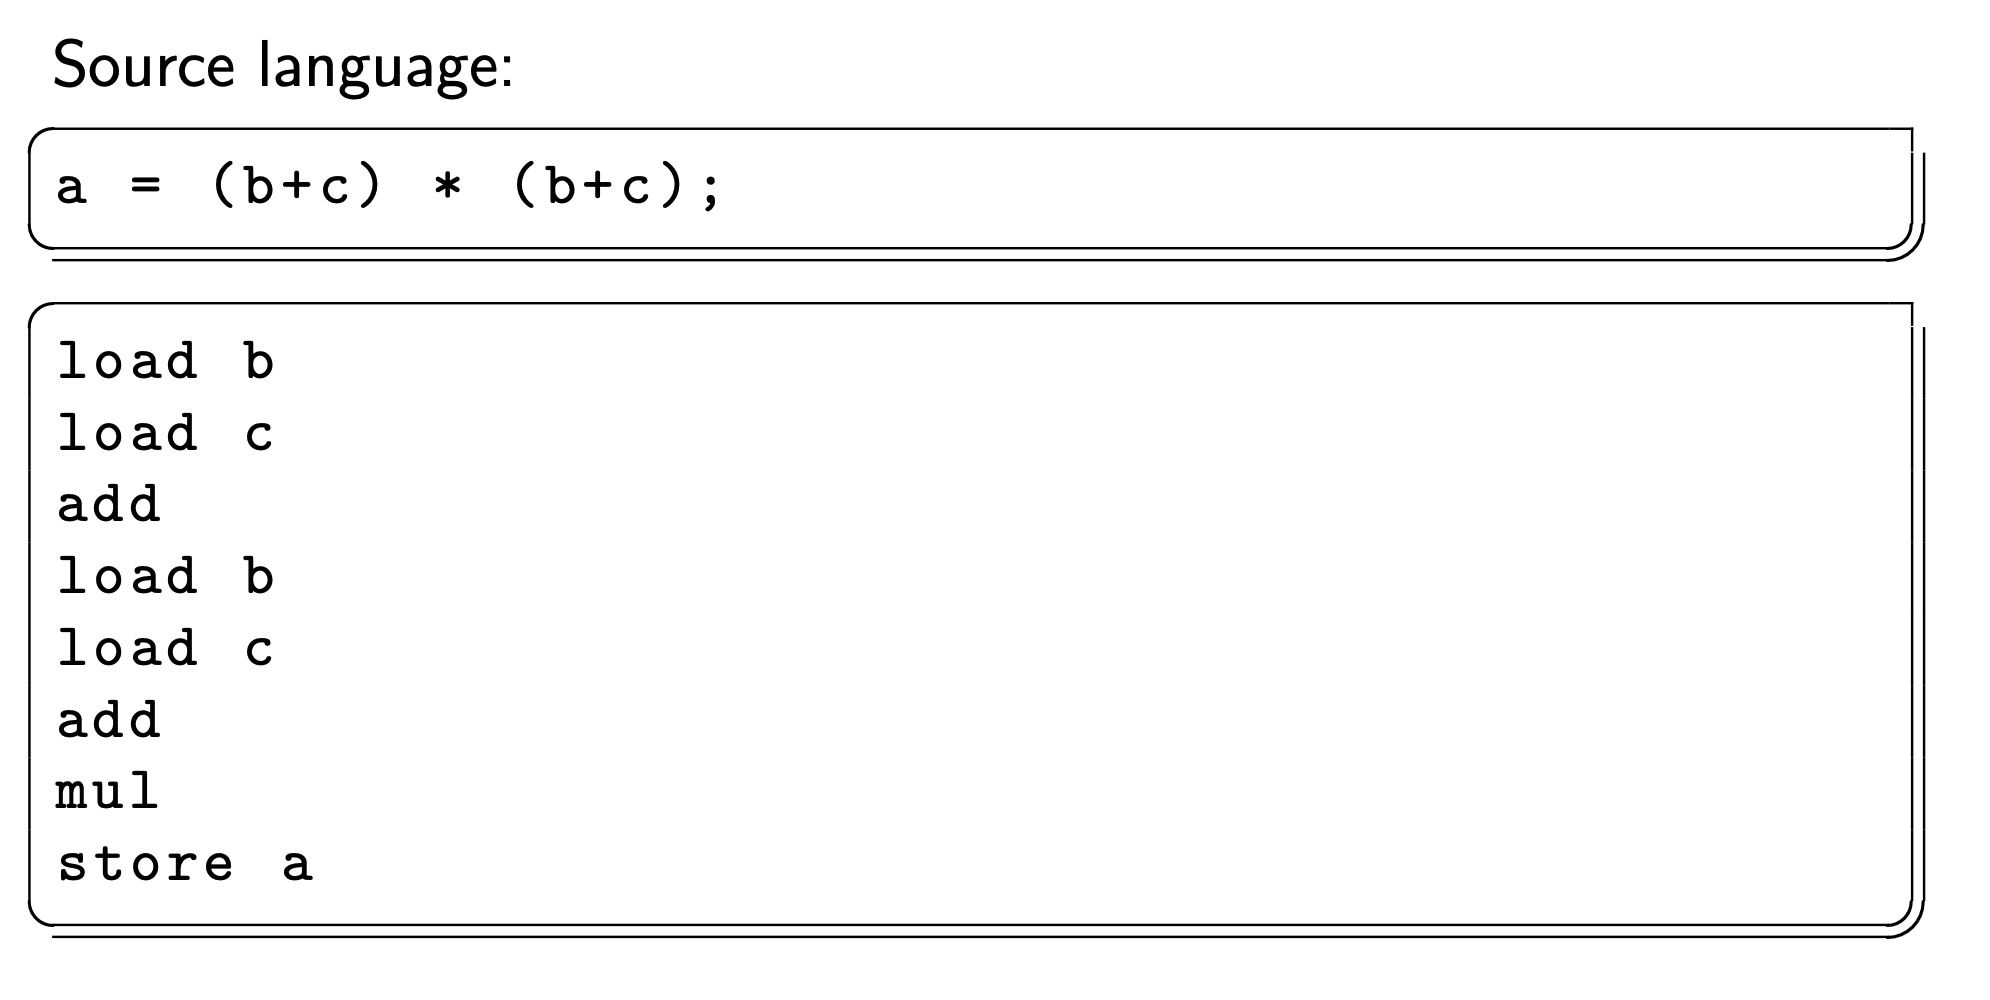
\includegraphics[height=3cm]{img/Snipaste_2021-04-05_17-27-00.png}
   \end{center}

\subsubsection{Problems with CSE and Stack IR}

\begin{enumerate}
  \item Entire operation must happen at once (no incremental algorithm)
  \item Finding identical subtrees is possible, reusing results is harder • If the operations were not adjacent, must spill to temporary
\end{enumerate}

\subsubsection{Hierarchical vs Flat IR}
\begin{enumerate}
  \item Source code is hierarchical (contains structured flow control, scoped values)
  \item Assembly is flat (all flow control is by jumps)
  \item Intermediate representations are supposed to be somewhere
  between the two
  \item Think about the possible ways that a for loop, while loop, and if statement with a backwards goto might be represented.
\end{enumerate}

\subsubsection{Hierarchical IR}
\begin{enumerate}
\item  Easy to express high-level constructs
\item Preserves program semantics
\item Preserves high-level semantics (variable lifetime, exceptions) clearly
\item Example: Ark Compiler, Flamming my compiler
\end{enumerate}
\subsection{Flat IR}

\begin{enumerate}
  \item Easy to map to the back end
  \item Simple for optimisations to process
  \item Must carry scope information in ad-hoc ways (e.g. LLVM IR has intrinsics to explicitly manage lifetimes for stack allocations)
  \item Examples: LLVM IR, CGIR, PTX
\end{enumerate}
\section{What Is LLVM IR?}
\begin{enumerate}
  \item Unlimited Single-Assignment Register machine instruction set • Strongly typed
  \item Three common representations:
  \item Human-readable LLVM assembly (.ll files)
  \item Dense ‘bitcode’ binary representation (.bc files) • C++ classes
\end{enumerate}

\subsection{Unlimited Register Machine?}

\begin{enumerate}
  \item  Real CPUs have a fixed number of registers
  \item LLVM IR has an infinite number
  \item New registers are created to hold the result of every instruction
  \item CodeGen’s register allocator determines the mapping from LLVM registers to physical registers
  \item Type legalisation maps LLVM types to machine types and so on (e.g. 128-element float vector to 32 SSE vectors or 16 AVX vectors, 1-bit integers to 32-bit values)
\end{enumerate}

\subsection{Static Single Assignment}
\begin{enumerate}
  \item Registers may be assigned to only once
  \item Most (imperative) languages allow variables to be... variable
  \item This requires some e↵ort to support in LLVM IR: SSA registers are not variables
  \item SSA form makes dataflow explicit: All consumers of the result of an instruction read the output register(s)
\end{enumerate}

\textbf{Example:}

\begin{center}
  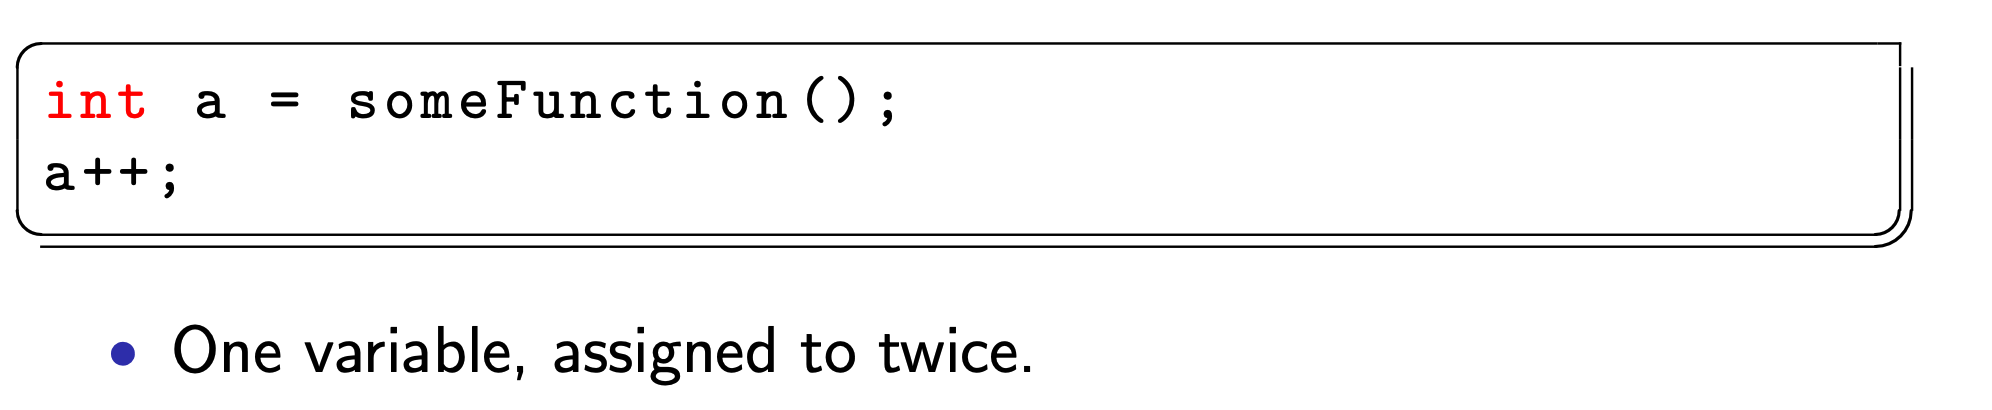
\includegraphics[height=1.7cm]{img/Snipaste_2021-04-05_17-33-40.png}
  \end{center}
\begin{center}
  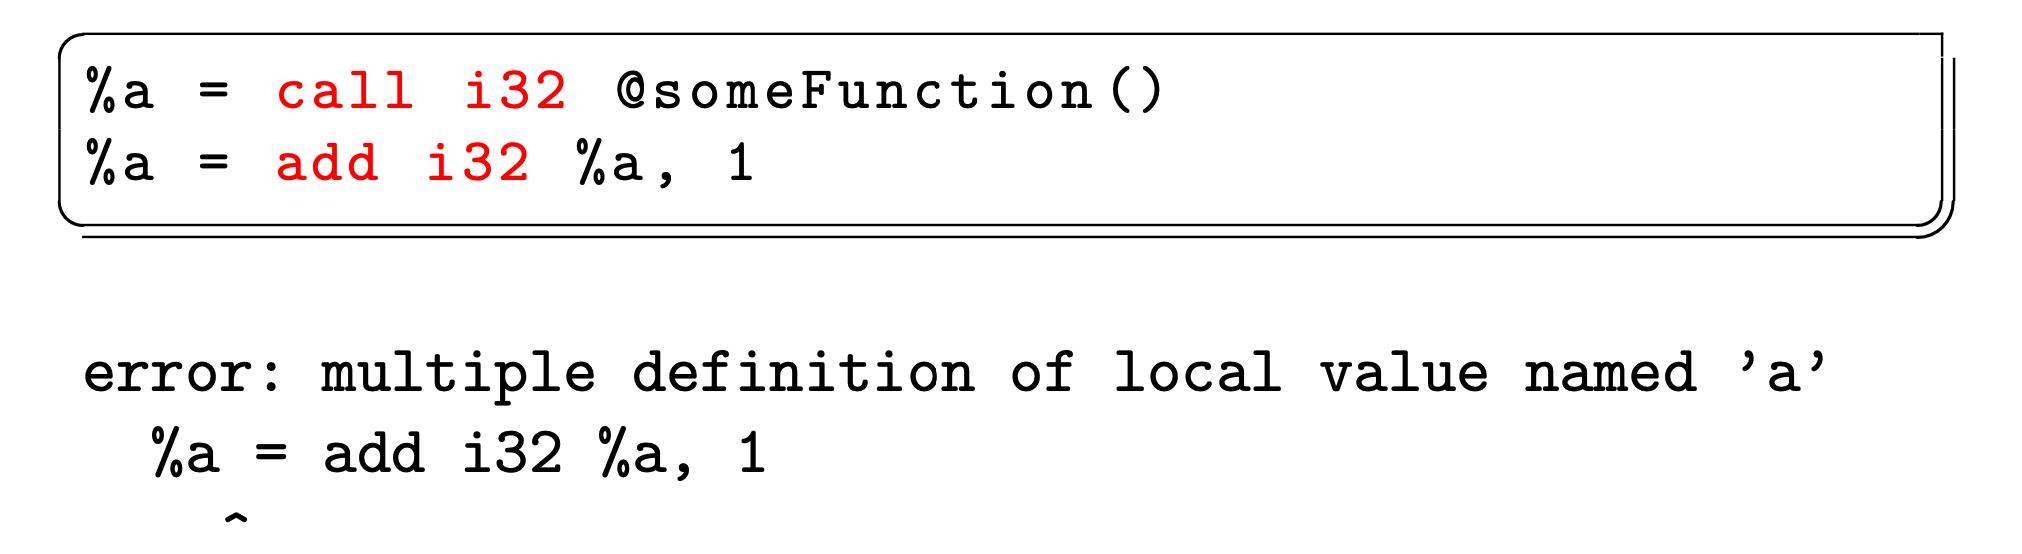
\includegraphics[height=2.5cm]{img/Snipaste_2021-04-05_17-34-02.png}
  \end{center}
\begin{center}
  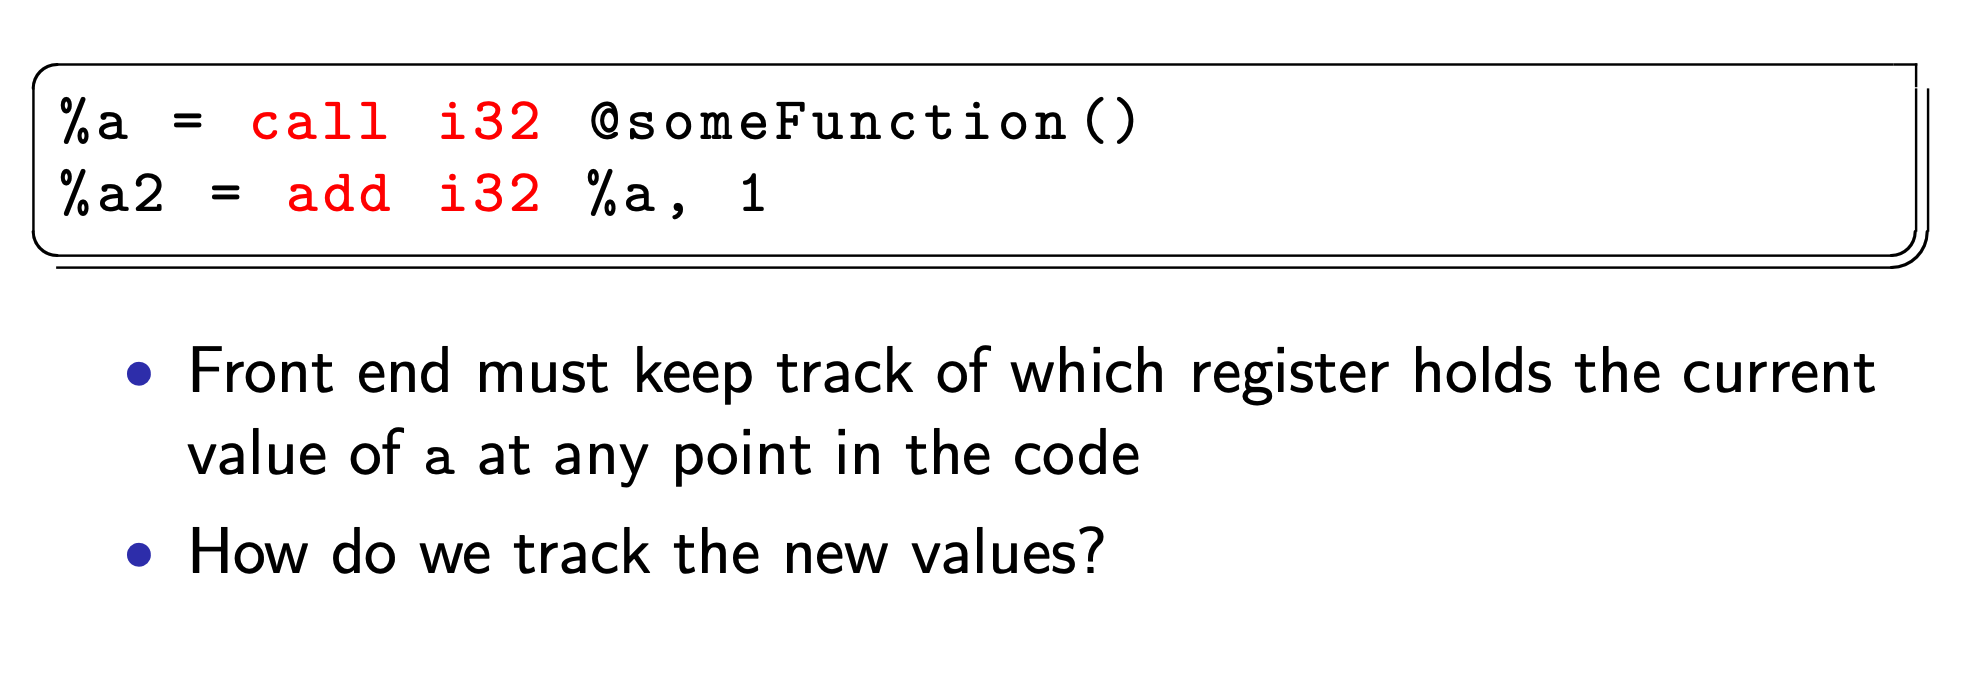
\includegraphics[height=3cm]{img/Snipaste_2021-04-05_17-34-41.png}
  \end{center}
  
  \subsection{Translating to LLVM IR The Easy Way}
  \begin{center}
    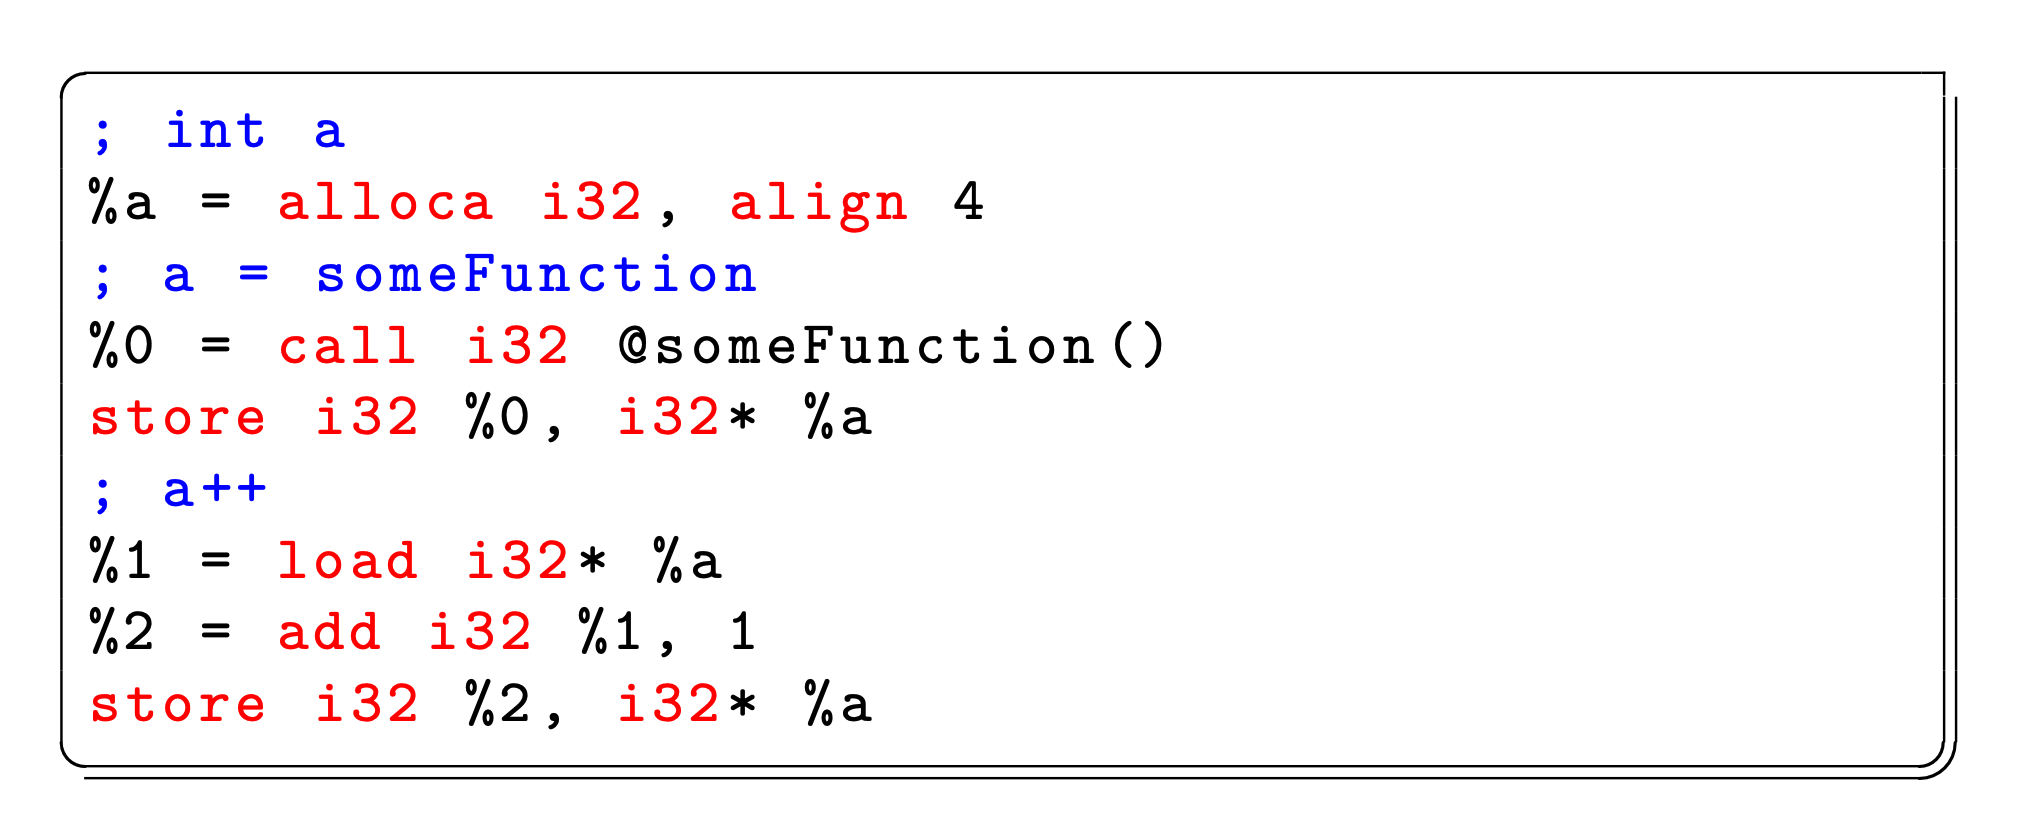
\includegraphics[height=3cm]{img/Snipaste_2021-04-05_17-35-19.png}
    \end{center}
    \begin{enumerate}
      \item Numbered register are allocated automatically
      \item  Each expression in the source is translated without worrying
      about data flow
      \item  Memory is not SSA in LLVM
    \end{enumerate}
    \subsubsection{Isn’t That Slow?}
    \begin{center}
      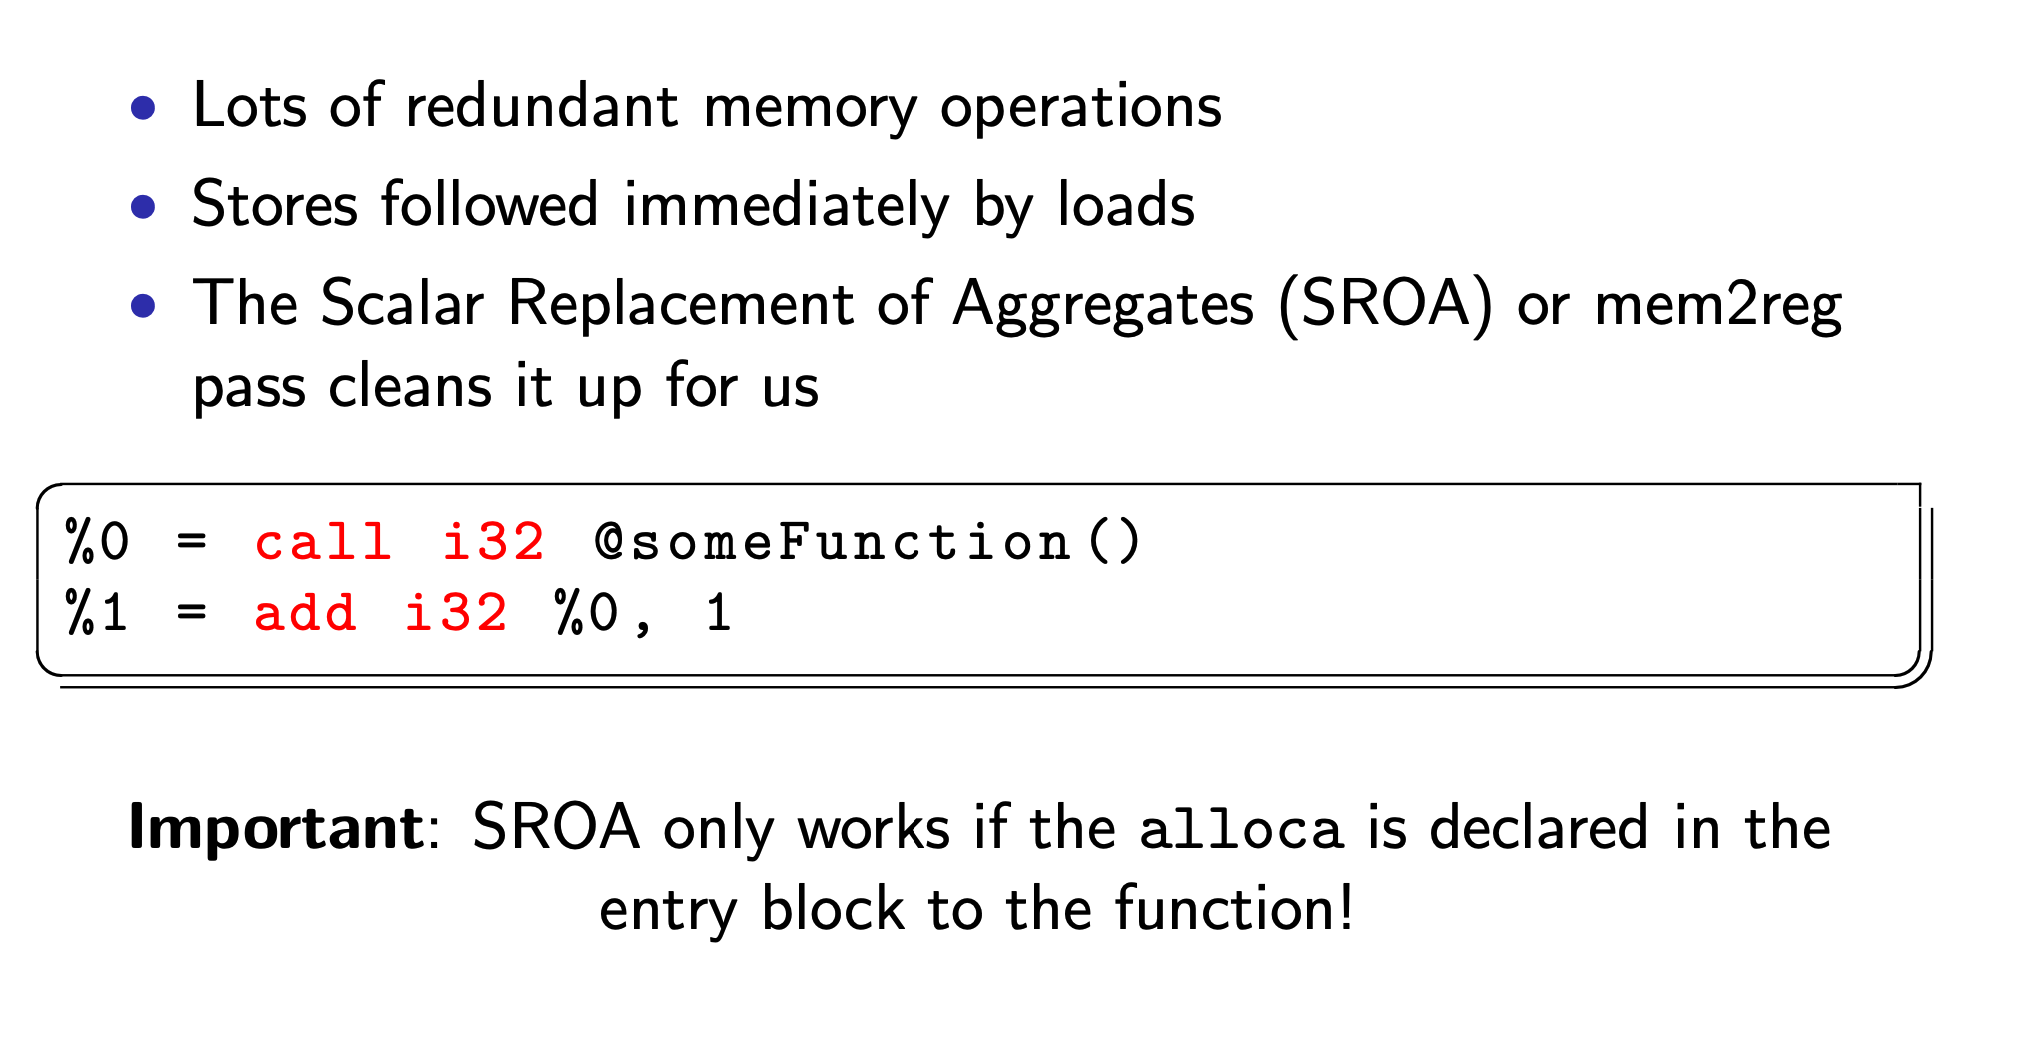
\includegraphics[height=6cm]{img/Snipaste_2021-04-05_17-37-34.png}
      \end{center}
\subsection{Sequences of Instructions}
\begin{enumerate}

  \item A sequence of instructions that execute in order is a basic block
  \item Basic blocks must end with a terminator
  \item Terminators are intraprocedural flow control instructions.
  \item call is not a terminator because execution resumes at the same place after the call
  \item invoke is a terminator because flow either continues or branches to an exception cleanup handler
  \item This means that even “zero-cost” exceptions can have a cost: they complicate the control-flow graph (CFG) within a function and make optimisation harder.
\end{enumerate}
\subsection{Intraprocedural Flow Control}
\begin{enumerate}
  \item Assembly languages typically manage flow control via jumps / branches (often the same instructions for inter- and intraprocedural flow)
  \item LLVM IR has conditional and unconditional branches
  \item Branch instructions are terminators (they go at the end of a
  basic block)
  \item Basic blocks are branch targets
  \item You can’t jump into the middle of a basic block (by the definition of a basic block)
\end{enumerate}

\subsection{‘Phi, my lord, phi!’ - Lady Macbeth, Compiler Developer}

\begin{enumerate}
  \item  $\phi$ nodes are special instructions used in SSA construction
  \item Their value is determined by the preceding basic block
  \item $\phi$ nodes must come before any non- $\phi$ instructions in a basic
  block
  \item In code generation, $\phi$ nodes become a requirement for one
  basic block to leave a value in a specific register.
  Alternate representation: named parameters to basic blocks
\end{enumerate}
\begin{center}
  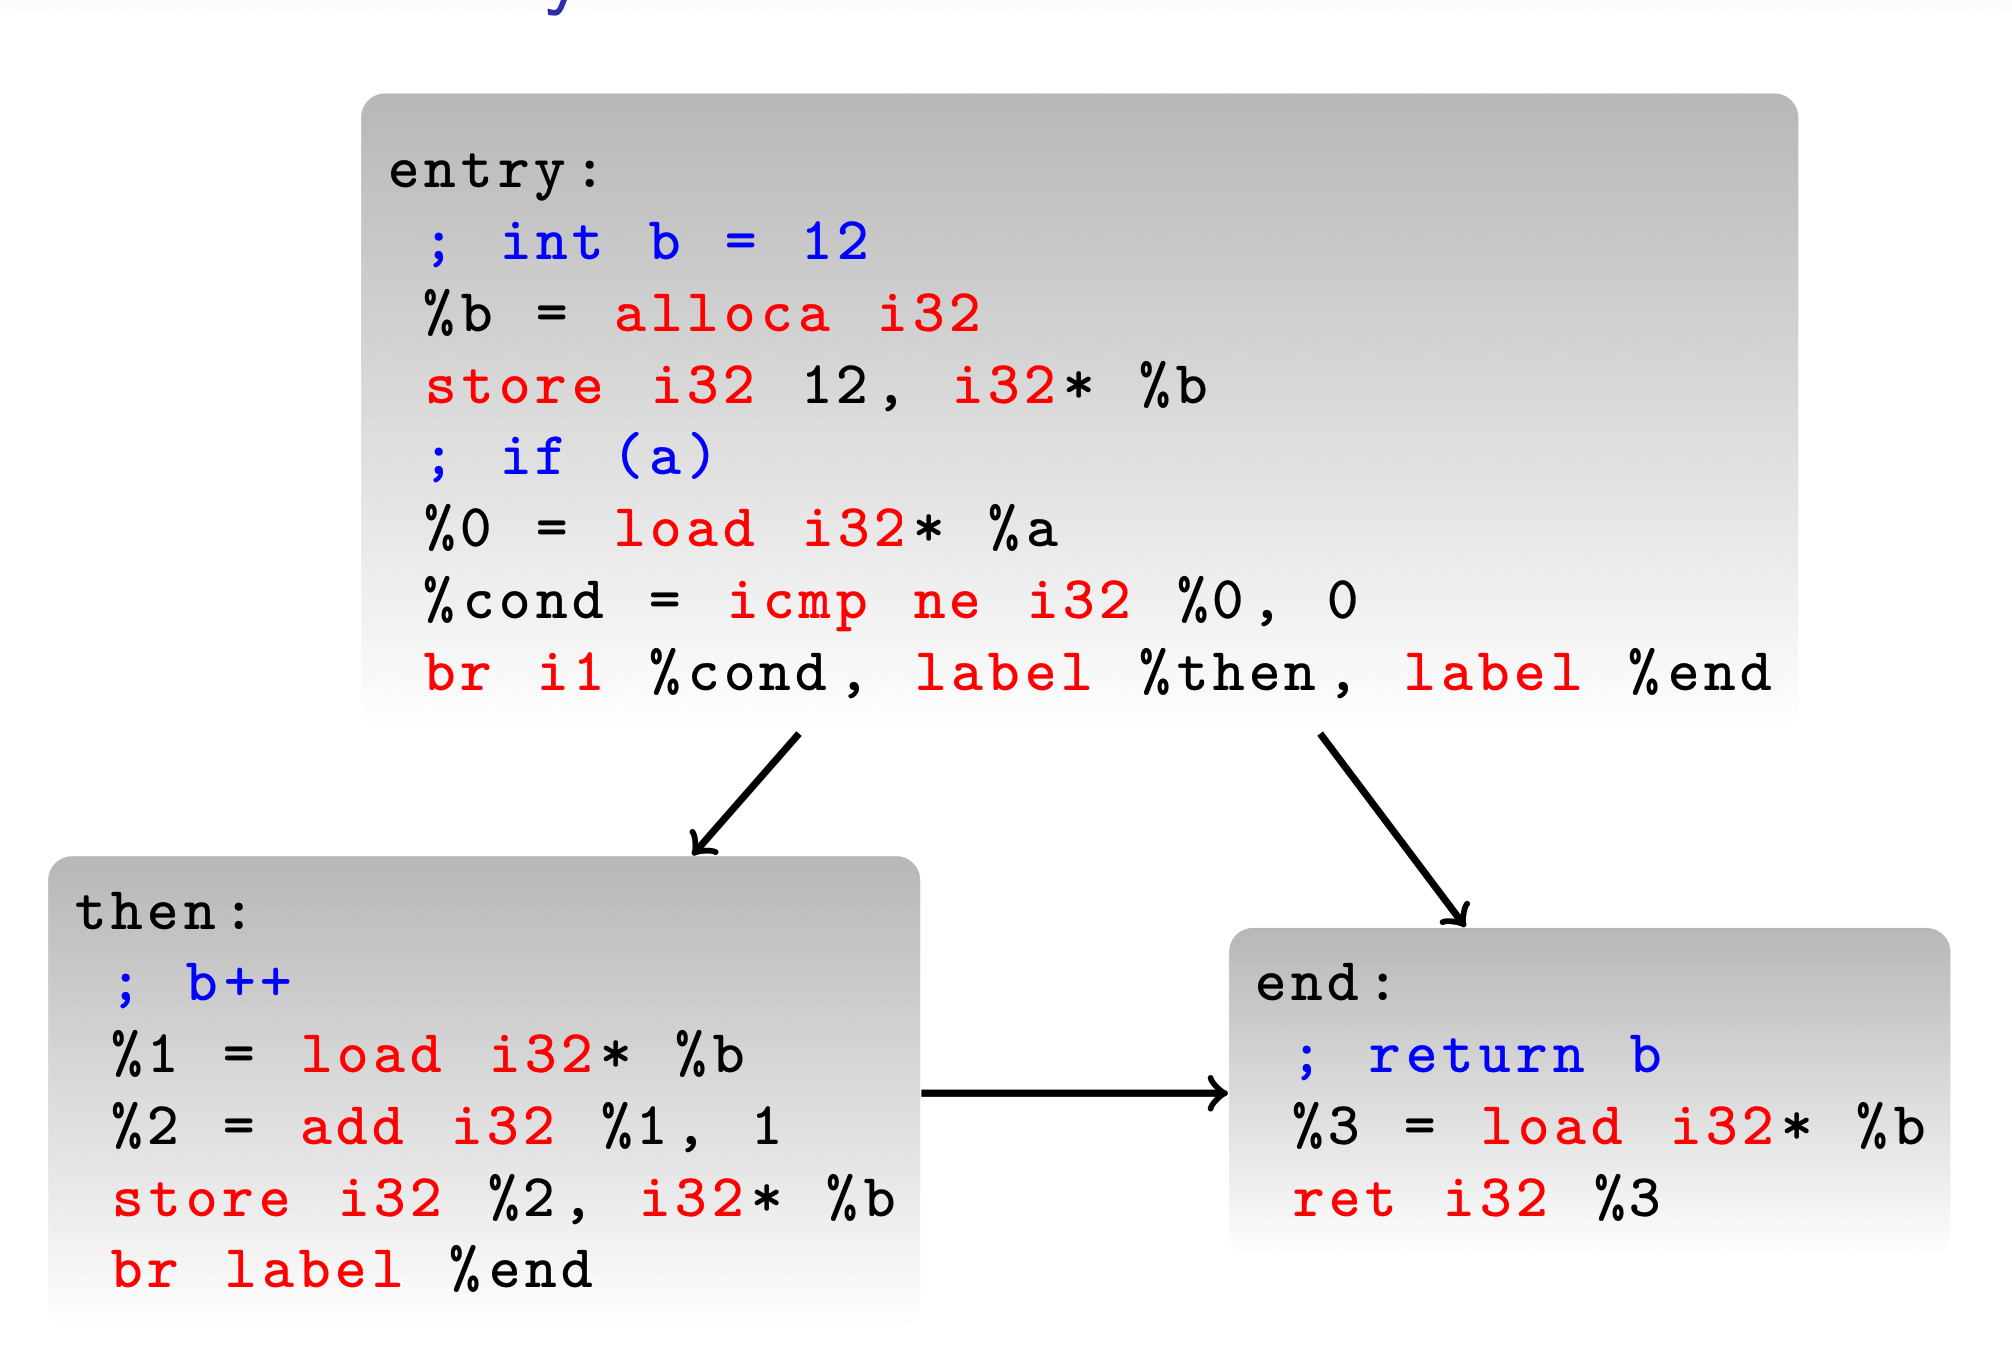
\includegraphics[height=6cm]{img/Snipaste_2021-04-05_17-40-27.png}
  \end{center}
  \subsection{Why Select?}
  \begin{center}
    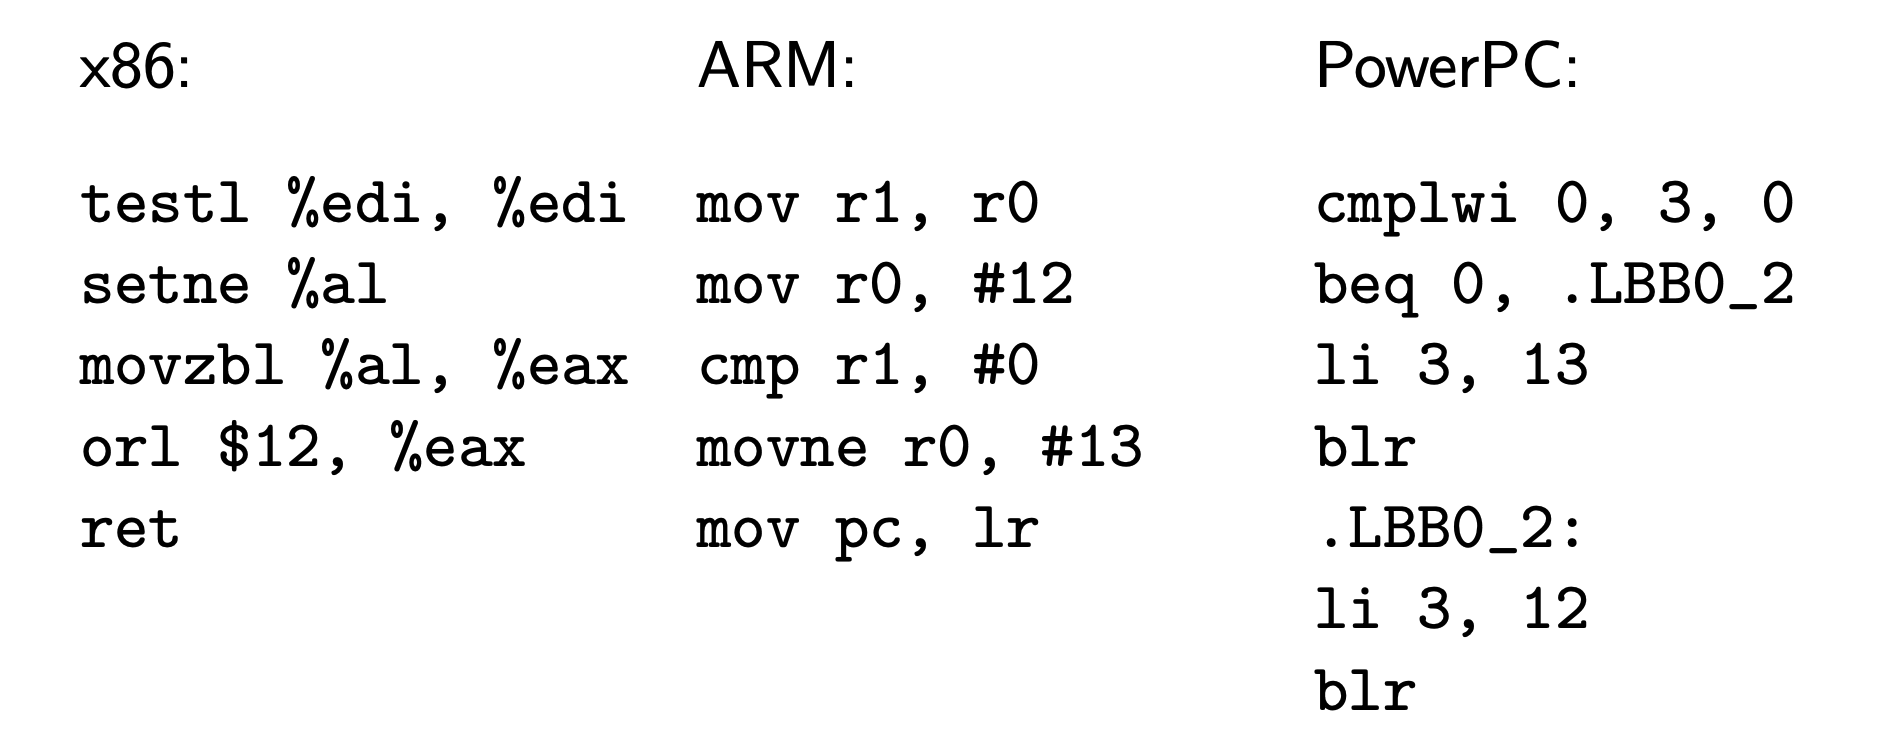
\includegraphics[height=6cm]{img/Snipaste_2021-04-05_17-41-52.png}
    \end{center}
    
    \subsection{Functions}
    \begin{center}
      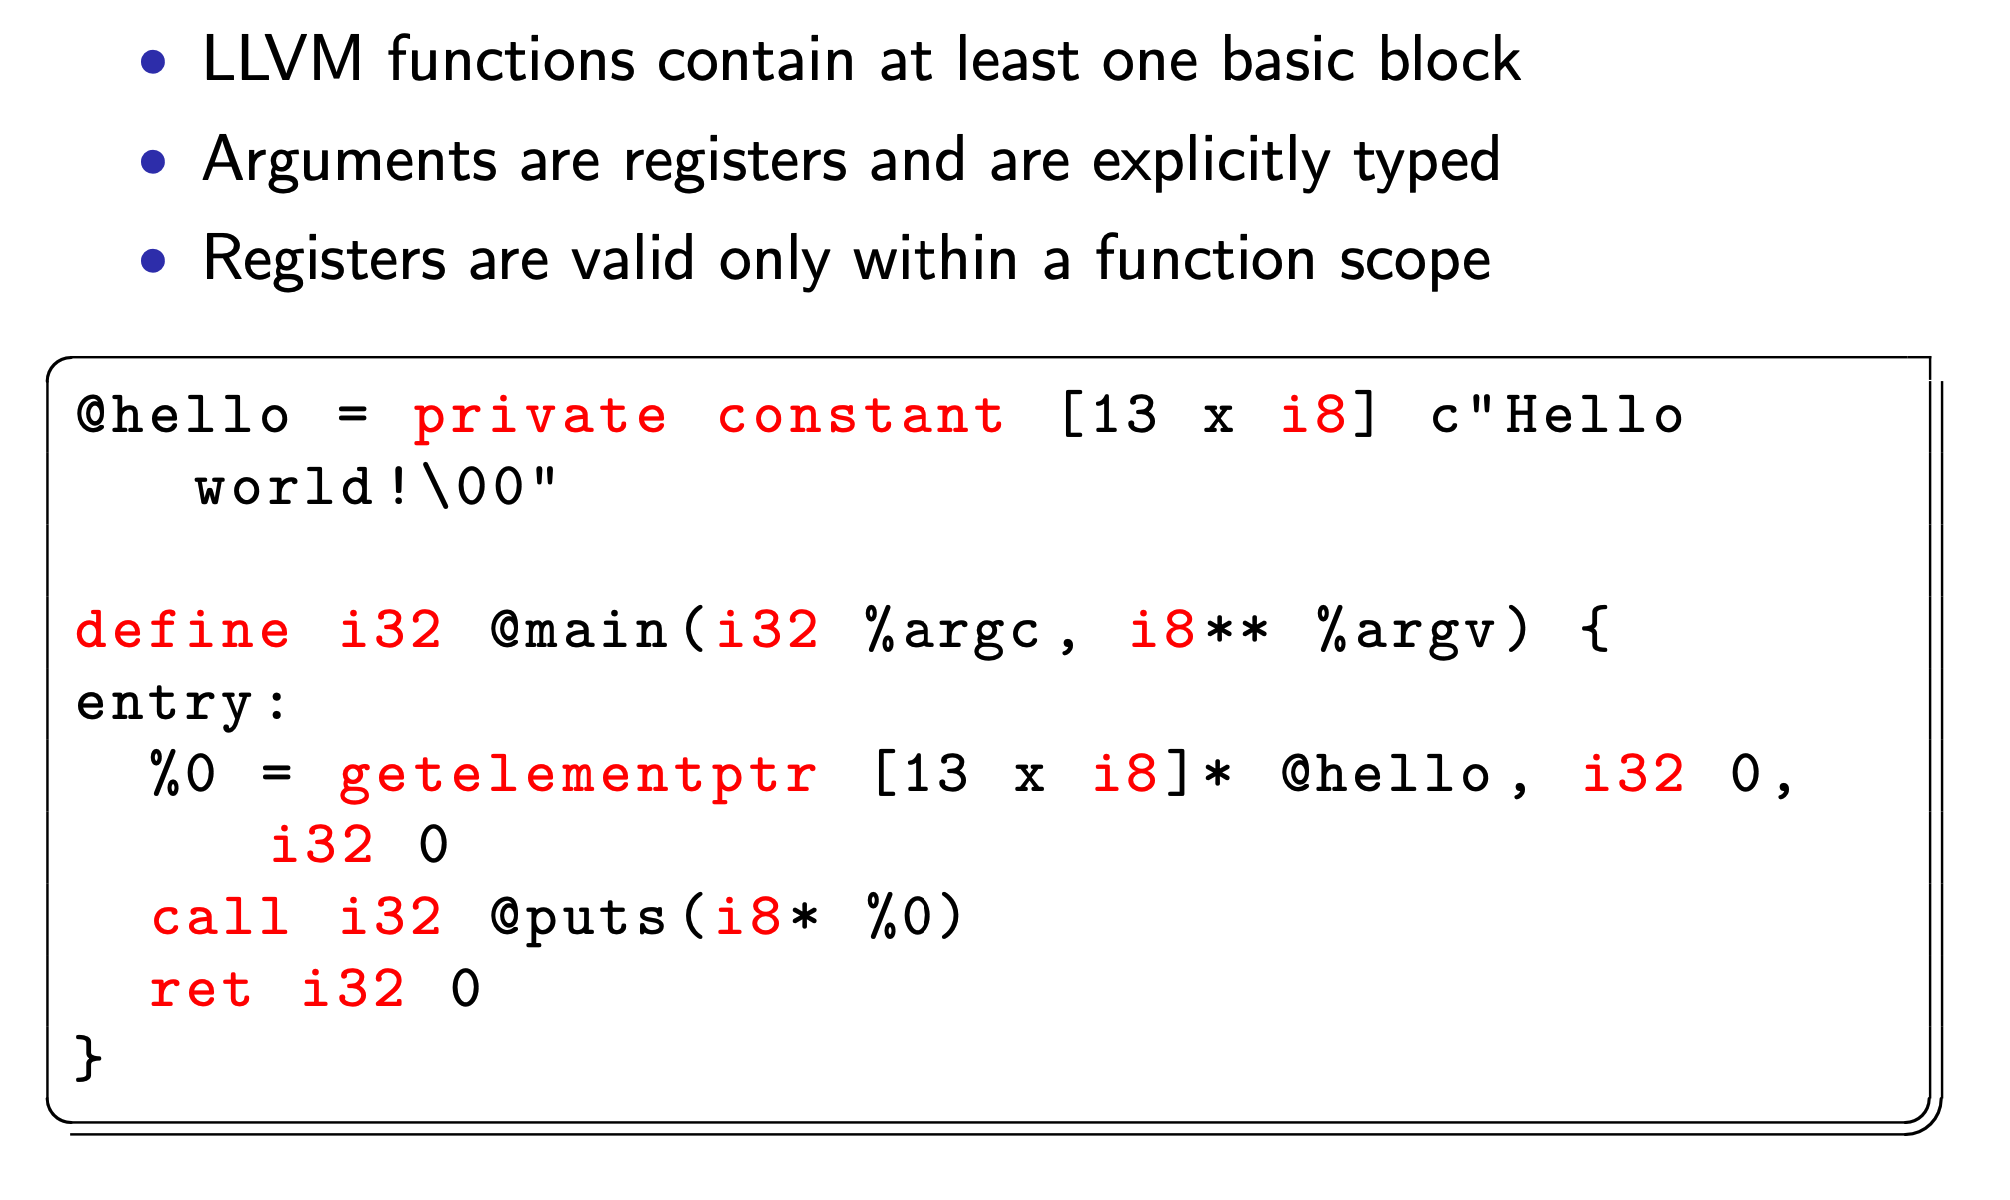
\includegraphics[height=6cm]{img/Snipaste_2021-04-05_17-42-34.png}
      \end{center}
\subsection{The Most Important LLVM Classes}

\begin{enumerate}
  \item Module - A compilation unit.
  \item Function - Can you guess?
  \item BasicBlock - a basic block
  \item GlobalVariable (I hope it’s obvious)
  \item IRBuilder - a helper for creating IR
  \item Type - superclass for all LLVM concrete types
  \item ConstantExpr - superclass for all constant expressions
  \item PassManagerBuilder - Constructs optimisation pass sequences to run
  \item ExecutionEngine - Interface to the JIT compiler
   
\end{enumerate}

\subsection{Writing A Simple Pass}
\begin{enumerate}
  \item Memoise an expensive library call
  \item Call maps a string to an integer (e.g. string intern function) • Mapping can be expensive.
  \item Always returns the same result.
\end{enumerate}

\subsection{Selection DAG}
\begin{enumerate}
  \item DAG defining operations and dependencies
  \item Legalisation phase lowers IR types to target types
  \begin{enumerate}
  \item Arbitrary-sized vectors to fixed-size
  \item Float to integer and softfloat library calls 
  \end{enumerate}
  
  \item DAG-to-DAG transforms simplify structure
  \item Code is still (more or less) architecture independent at this
  point
  \item Some peephole optimisations happen here
\end{enumerate}

\begin{center}
  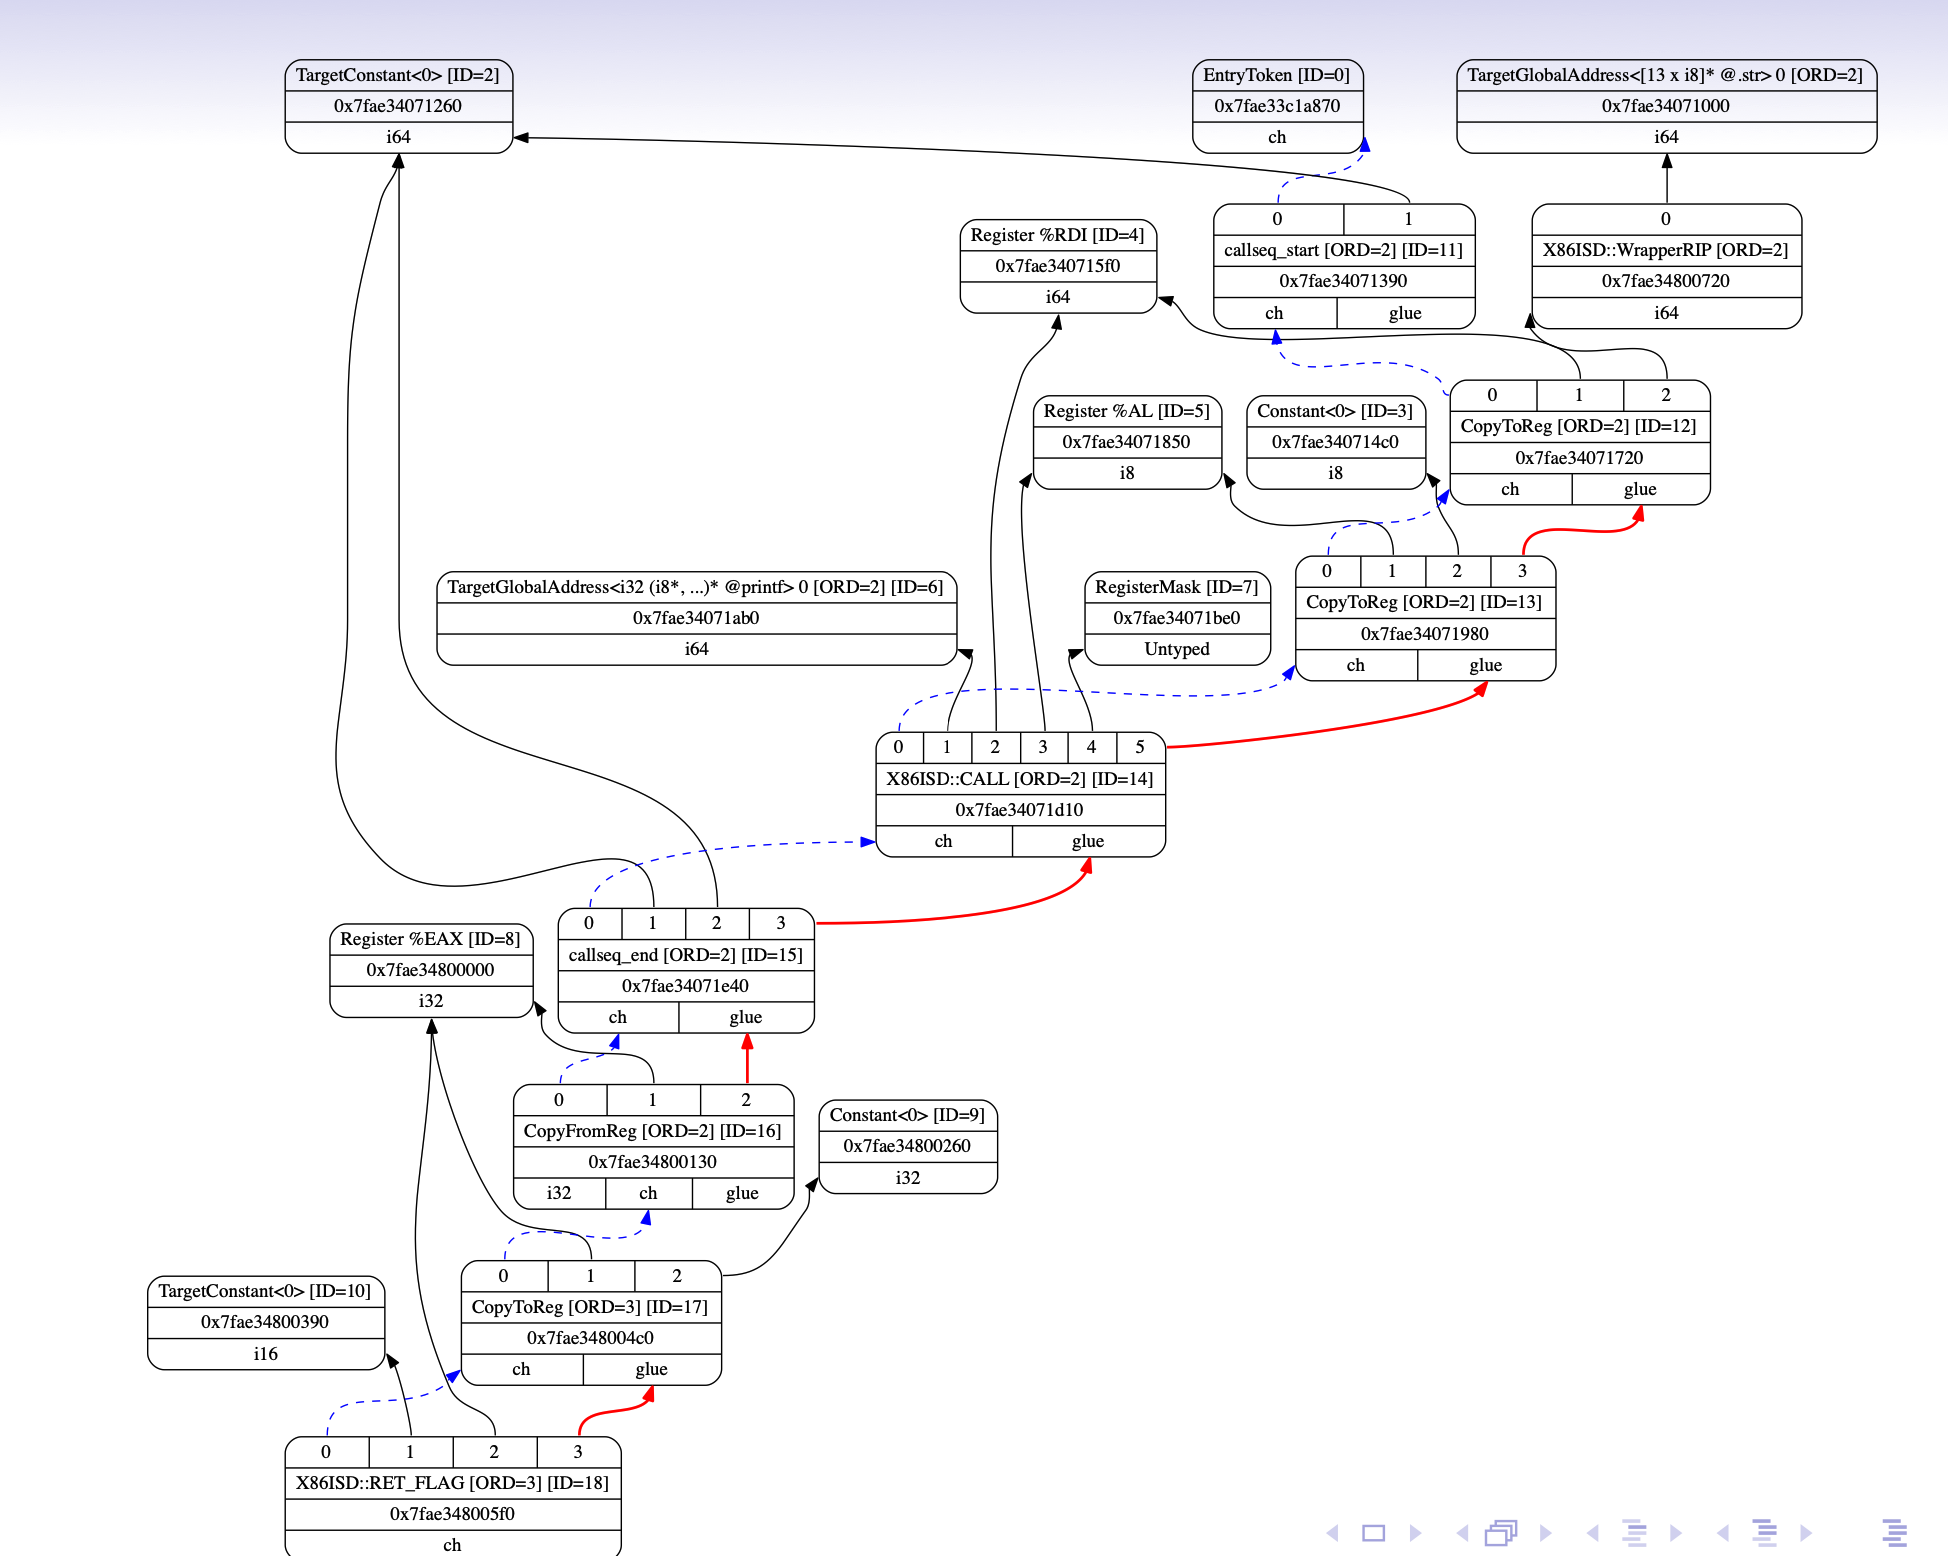
\includegraphics[height=12cm]{img/Snipaste_2021-04-05_17-45-22.png}
  \end{center}
\end{document}
